\section{Proposed System: ULP-V2V-Auth}

\subsection{System Model}

The ULP-V2V-Auth system consists of four entity types:

\begin{itemize}
    \item \textbf{Trusted Authority (TA):} A trusted offline entity responsible for
    registering vehicles, issuing long-term anonymous credentials, maintaining the
    Merkle tree of active ASTs, and handling revocation decisions.
    \item \textbf{AST Issuing Service (AIS):} An infrastructure service
    (co-located with RSUs or accessible via cellular networks) that issues
    short-lived Anonymous Session Tokens upon presentation of valid long-term
    credentials. The AIS is authenticated to vehicles via a TA-signed certificate
    (Section~\ref{sec:ast_issuance}).
    \item \textbf{Prover Vehicle ($V_P$):} A vehicle holding a valid AST that
    generates ZKP proofs to authenticate its safety messages, performing offline
    precomputation during AST acquisition and lightweight online proof generation
    per message.
    \item \textbf{Verifier Vehicle ($V_V$):} A receiving vehicle that collects
    incoming safety messages with attached ZKP proofs and performs batch
    verification to authenticate multiple messages simultaneously.
\end{itemize}

The communication model assumes direct V2V sidelink (IEEE 802.11p/802.11bd or
C-V2X Mode~4) for safety message exchange, and intermittent infrastructure access
(RSU, cellular, or Wi-Fi) for AST acquisition and Merkle root updates.

\begin{figure}[t]
    \centering
    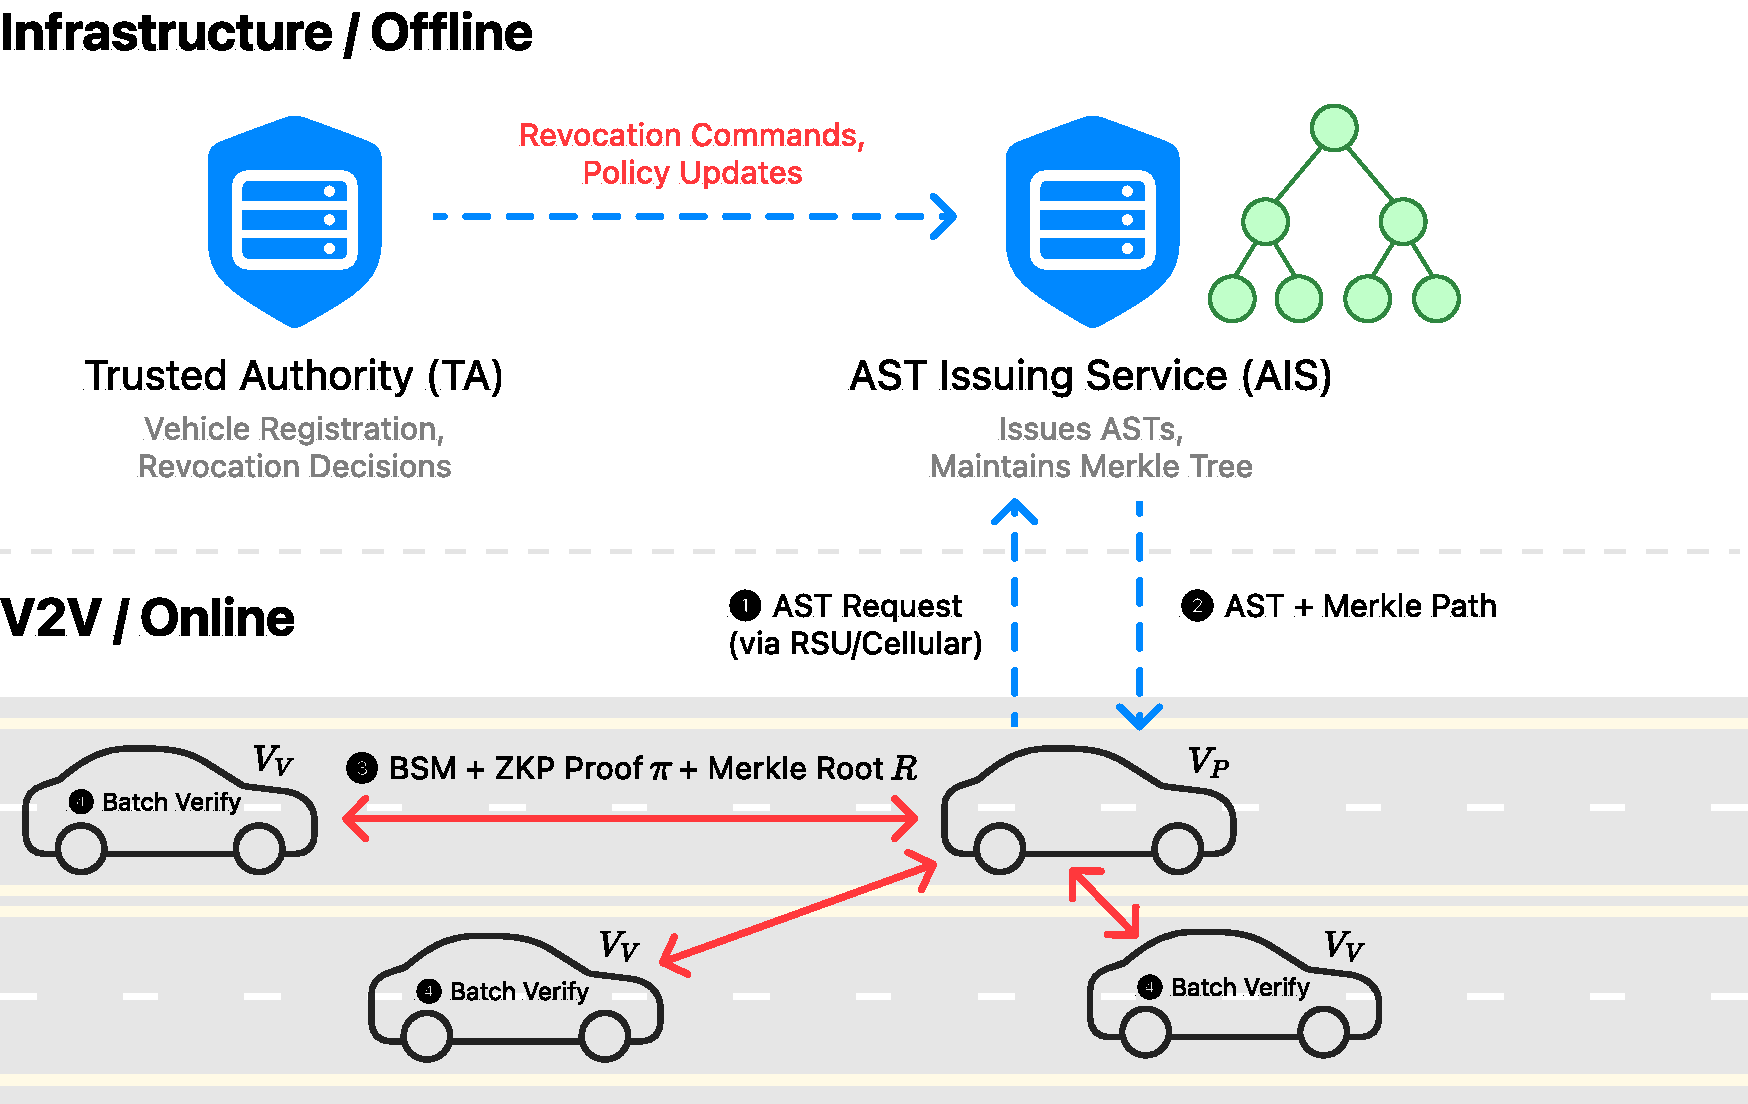
\includegraphics[width=\linewidth]{assets/system_model.pdf}
    \caption{System model of ULP-V2V-Auth showing the four entities and their
    interactions across offline (AST acquisition) and online (V2V authentication)
    phases.}
    \label{fig:system_model}
\end{figure}

\subsection{Cryptographic Preliminaries}

\subsubsection{Bilinear Pairing}
Let $\mathbb{G}_1$, $\mathbb{G}_2$, and $\mathbb{G}_T$ be cyclic groups of prime
order $p$. A bilinear pairing is a map $e: \mathbb{G}_1 \times \mathbb{G}_2
\rightarrow \mathbb{G}_T$ satisfying bilinearity ($e(aP, bQ) = e(P, Q)^{ab}$),
non-degeneracy, and efficient computability. We use the BN254 elliptic curve,
providing approximately 128-bit security and efficient pairing computation.

\subsubsection{Groth16 zk-SNARK}
Groth16~\cite{groth2016} is a pairing-based zk-SNARK producing proofs of only three
group elements $(A \in \mathbb{G}_1, B \in \mathbb{G}_2, C \in \mathbb{G}_1)$,
yielding a proof size of $\approx$128 bytes on BN254. Verification requires exactly
3 pairing operations and is constant-time regardless of circuit size. The system
consists of three algorithms: $\mathsf{Setup}(\mathcal{C}) \rightarrow (\mathsf{pk},
\mathsf{vk})$; $\mathsf{Prove}(\mathsf{pk}, x, w) \rightarrow \pi$; and
$\mathsf{Verify}(\mathsf{vk}, x, \pi) \rightarrow \{0, 1\}$.

\subsubsection{Merkle Hash Tree}
A Merkle hash tree is a binary tree where each leaf contains the hash of a data block
and each internal node contains the hash of its two children. A membership proof
(Merkle path) for a tree with $n$ leaves consists of $\lceil \log_2 n \rceil$ hash
values. We use the Poseidon hash function~\cite{poseidon2021}, optimized for
arithmetic circuits (SNARK-friendly), requiring significantly fewer constraints
than SHA-256 when embedded in a ZKP circuit.

\subsection{Protocol Design}

The ULP-V2V-Auth protocol operates in four phases, as illustrated in
Fig.~\ref{fig:protocol_flow}.

\begin{figure}[t]
    \centering
    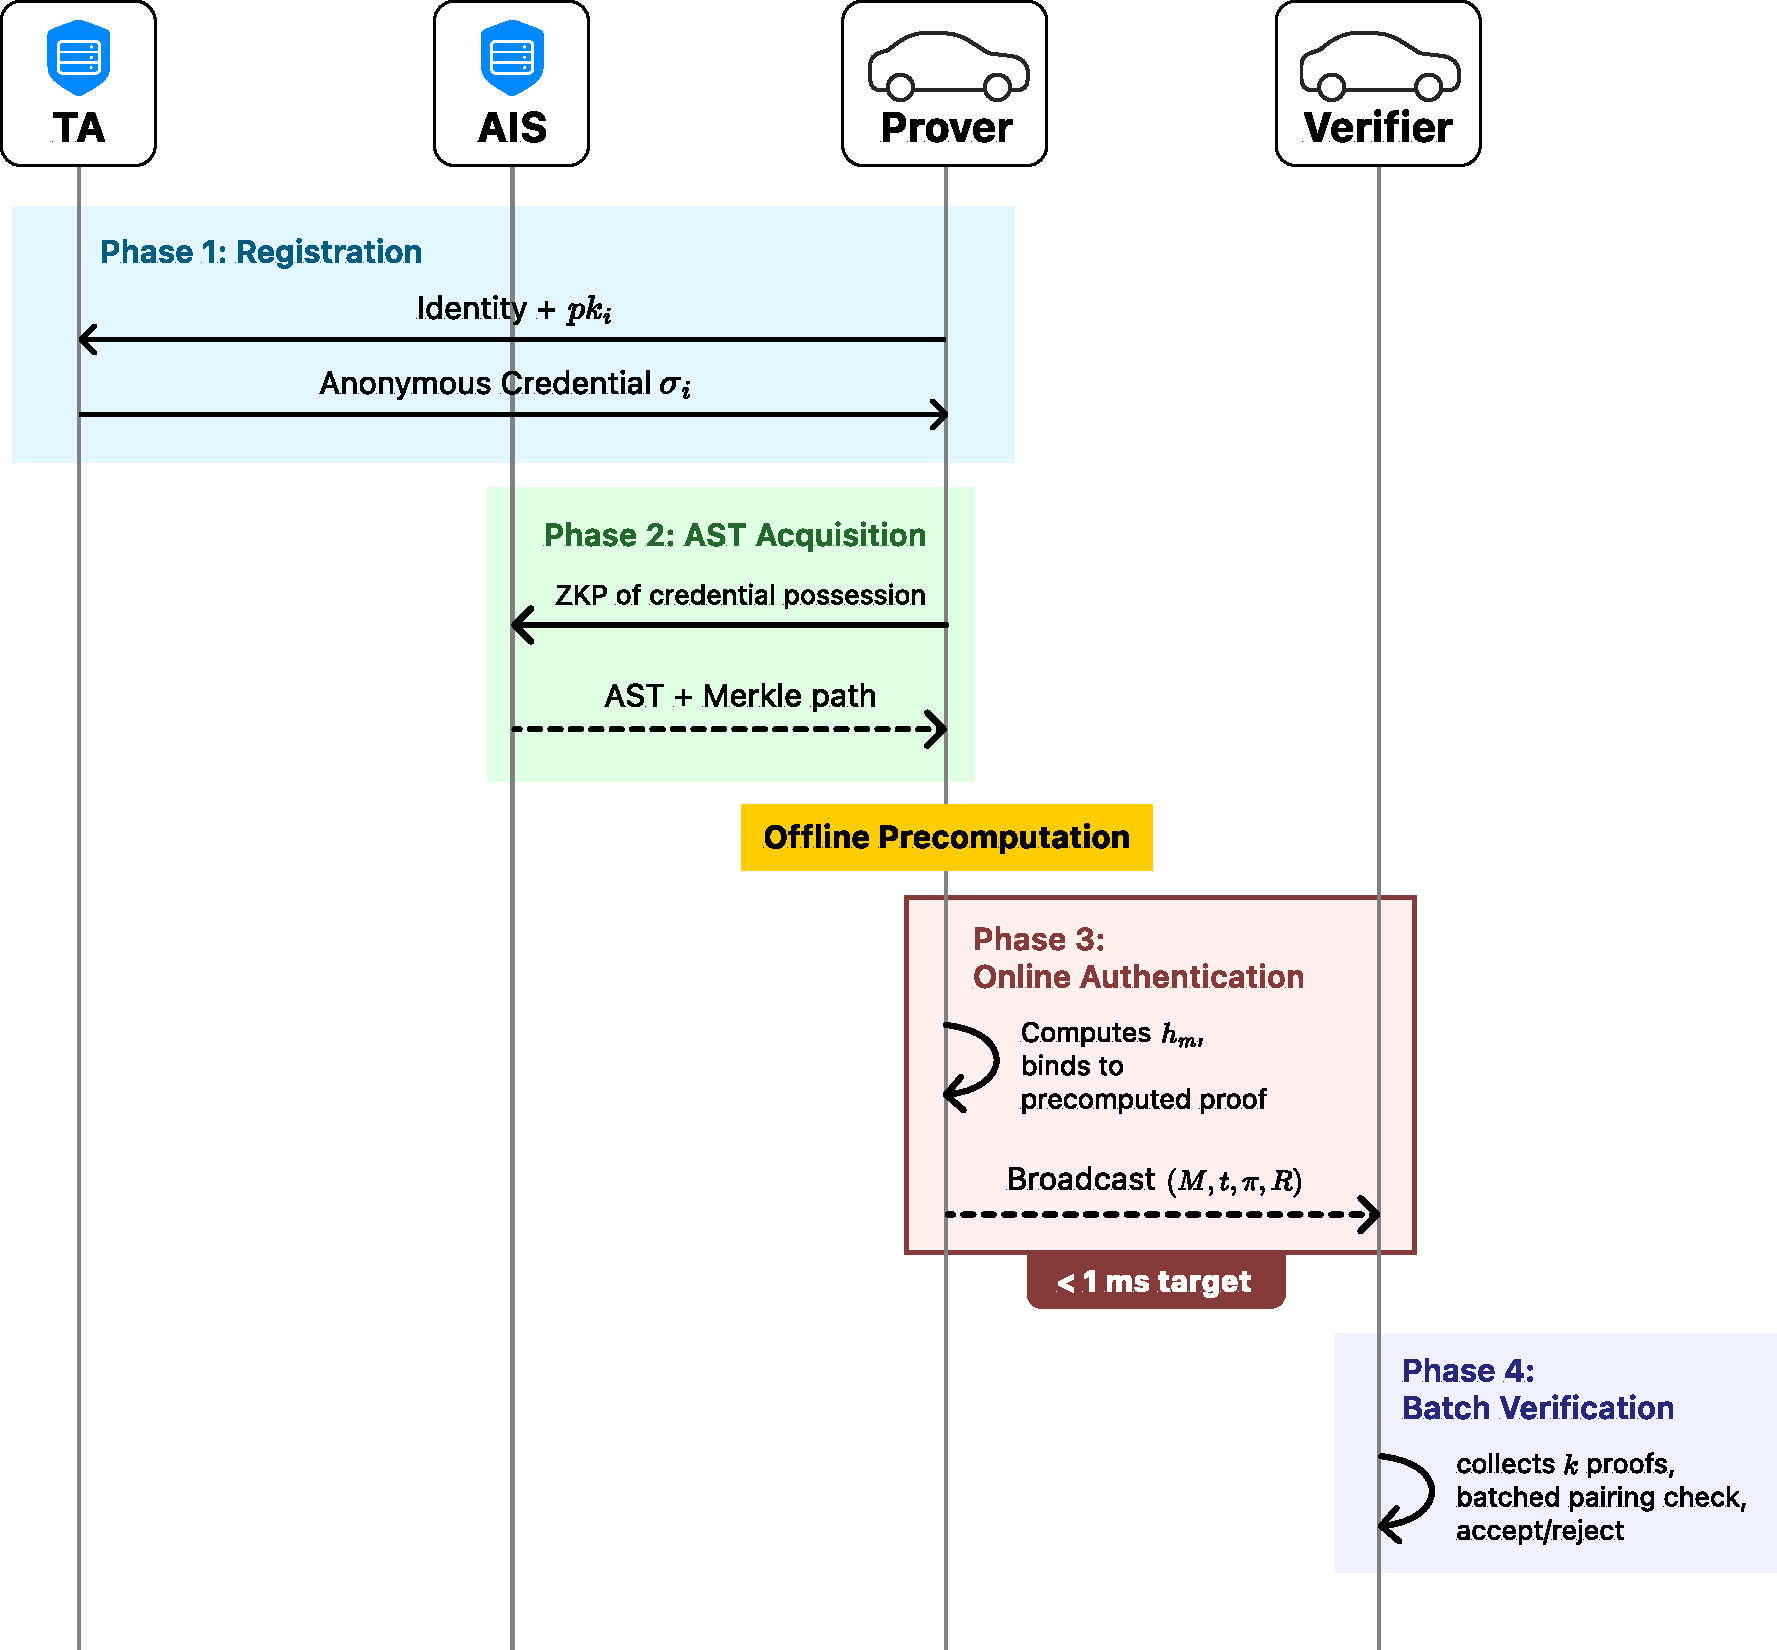
\includegraphics[width=\linewidth]{assets/seqdia.pdf}
    \caption{Protocol flow of ULP-V2V-Auth showing the four phases: (1) Registration,
    (2) AST Acquisition, (3) Online Authentication, and (4) Batch Verification.}
    \label{fig:protocol_flow}
\end{figure}

\subsubsection{Phase 1: Vehicle Registration (One-Time)}
A vehicle $V_i$ registers with the TA through a secure out-of-band channel (Fig.~\ref{fig:phase1}):
\begin{enumerate}
    \item $V_i$ generates a long-term key pair $(sk_i, pk_i)$ on the BN254 curve.
    \item $V_i$ presents its real-world identity (e.g., VIN) and $pk_i$ to the TA.
    \item The TA verifies the vehicle's legitimacy and issues an anonymous credential
    $\sigma_i = \mathsf{Sign}_{sk_{TA}}(H(pk_i \| \mathsf{nonce}))$ via blind
    signature, attesting to $V_i$'s legitimacy without being linkable to $V_i$'s
    real identity by any party other than the TA.
    \item $V_i$ stores $(sk_i, \sigma_i, pk_{TA})$ securely in its OBU's
    tamper-proof module.
\end{enumerate}

\begin{figure}[t]
    \centering
    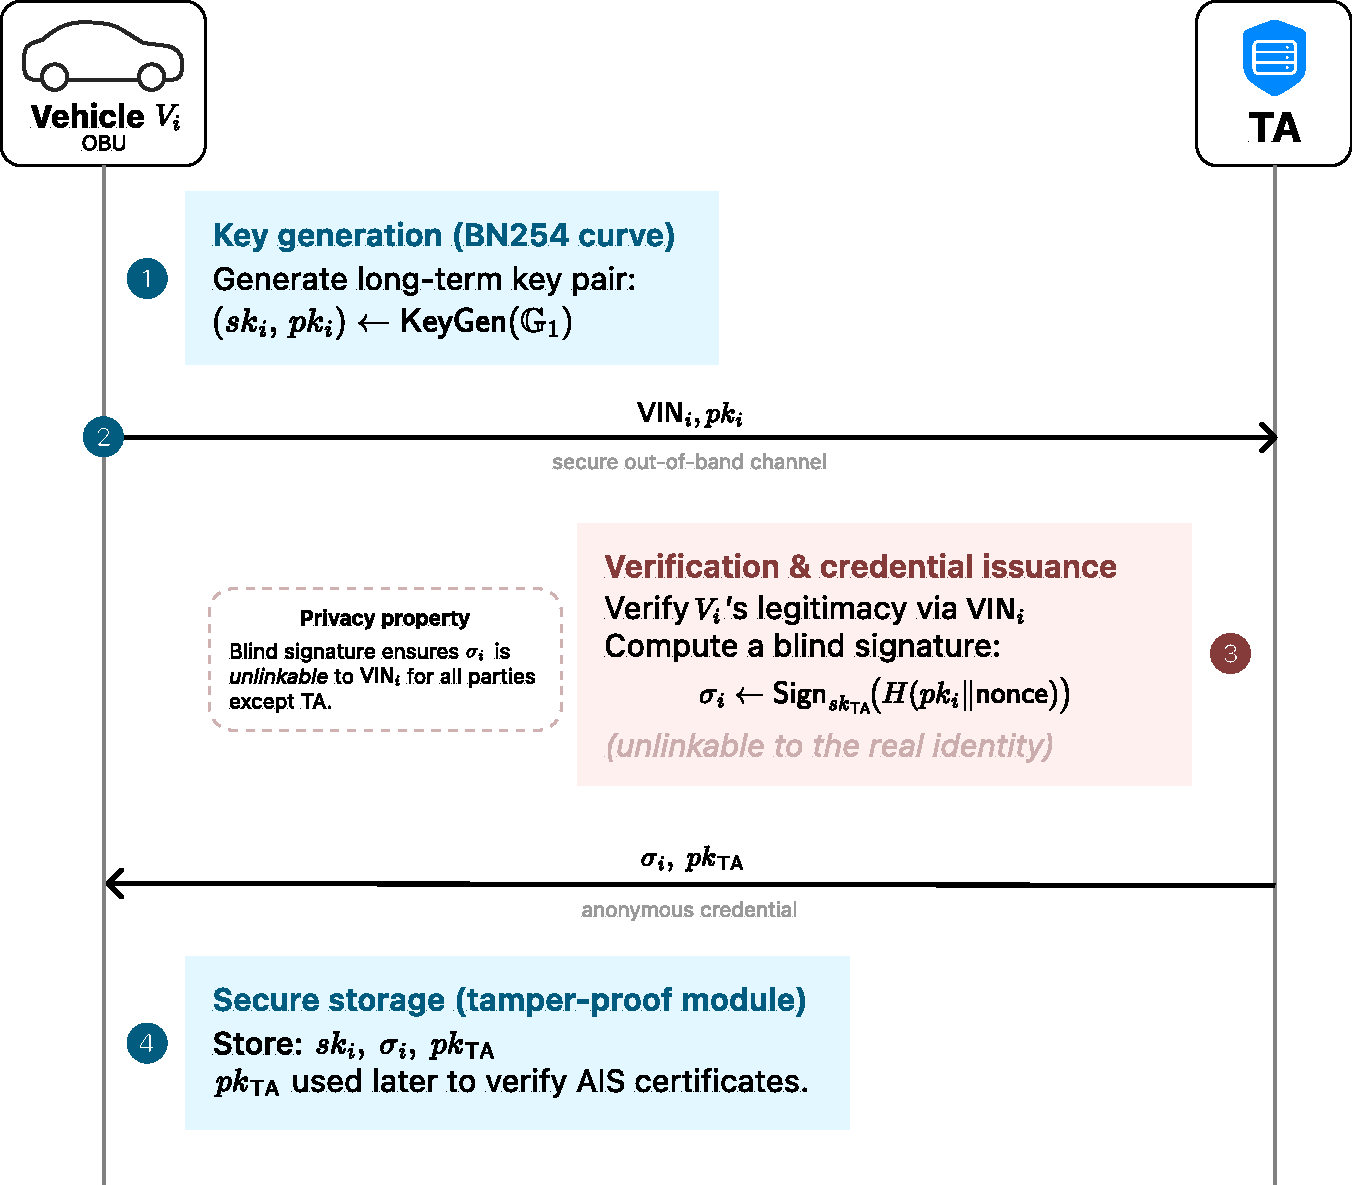
\includegraphics[width=\linewidth]{assets/phase1.pdf}
    \caption{Phase 1: Vehicle registration. $V_i$ submits $pk_i$ to the Trusted
    Authority, which issues an anonymous credential $\sigma_i$ via blind signature.
    The TA's public key $pk_{TA}$ is pre-loaded into the OBU for subsequent AIS
    certificate verification.}
    \label{fig:phase1}
\end{figure}

\begin{algorithm}[t]
\caption{Vehicle Registration --- Phase 1 (One-Time)}
\label{alg:registration}
\begin{algorithmic}[1]
\REQUIRE Vehicle identity $\mathsf{VIN}$, BN254 curve parameters, TA public key $pk_{TA}$
\ENSURE $(sk_i, pk_i, \sigma_i, pk_{TA})$ stored in OBU tamper-proof module
\STATE $(sk_i, pk_i) \leftarrow \mathsf{KeyGen}(\mathsf{BN254})$
\STATE Send $(\mathsf{VIN},\; pk_i)$ to TA over secure out-of-band channel
\STATE \textbf{[TA side]} Verify $\mathsf{VIN}$ legitimacy; abort if invalid
\STATE \textbf{[TA side]} $\mathsf{nonce} \xleftarrow{\$} \{0,1\}^{256}$
\STATE \textbf{[TA side]} $\sigma_i \leftarrow \mathsf{Sign}_{sk_{TA}}\!\bigl(H(pk_i \;\|\; \mathsf{nonce})\bigr)$
\STATE \textbf{[TA side]} Transmit $\sigma_i$ to $V_i$ over secure channel
\STATE $V_i$ verifies $\sigma_i$ against $pk_{TA}$; abort if invalid
\STATE Store $(sk_i,\; \sigma_i,\; pk_{TA})$ in OBU tamper-proof module
\end{algorithmic}
\end{algorithm}

\subsubsection{Phase 2: AST Acquisition (Periodic, Offline)}
When $V_i$ has infrastructure access, it requests a fresh AST per
Section~\ref{sec:ast_policy} (Fig.~\ref{fig:phase2}):
\begin{enumerate}
    \item $V_i$ connects to the AIS and verifies $\mathsf{cert}_{AIS}$ against
    $pk_{TA}$. If verification fails, the session is aborted.
    \item $V_i$ presents a ZKP of possession of valid credential $\sigma_i$,
    without revealing $\sigma_i$ or $pk_i$.
    \item The AIS generates an AST:
    $\mathsf{AST}_i = \{sid_i,\ t_{start},\ t_{end},\ cap_i,\ r_i\}$,
    where $sid_i$ is a random session identifier, $[t_{start}, t_{end}]$ spans at
    least two epochs, $cap_i$ encodes vehicle capabilities, and $r_i$ is a random
    blinding factor.
    \item The AIS computes
    $\mathsf{leaf}_i = H_{Poseidon}(sid_i \| t_{start} \| t_{end} \| cap_i \| r_i)$,
    inserts it into the Merkle tree, and returns $(R_{new}, \pi^{MT}_i,
    \mathsf{sig}_{AIS}, R_{next})$ to $V_i$, all signed as
    $\mathsf{sig}_{AIS} = \mathsf{Sign}_{sk_{AIS}}(H(R_{new} \| \pi^{MT}_i))$.
    \item \textbf{Offline Precomputation (Proof-Slot Cache):} $V_i$ precomputes
    $N_{cache}$ \emph{complete} Groth16 proofs, each committed to a predicted BSM
    content $(m^{(s)}_{\mathit{pred}}, t^{(s)}_{\mathit{pred}})$ for the next
    driving segment. Each slot stores the complete proof $\pi^{(s)}$ and its public
    inputs $(R,\; t^{(s)}_{\mathit{pred}},\; h^{(s)}_{m})$ where
    $h^{(s)}_{m} = H_{\mathit{Poseidon}}(m^{(s)}_{\mathit{pred}} \|
    t^{(s)}_{\mathit{pred}})$. The 97.3\% of circuit constraints that are
    message-independent (Merkle path, AST fields, timestamp range) make
    offline precomputation the dominant cost; only the per-slot message commitment
    varies between slots.
\end{enumerate}

\begin{figure}[t]
    \centering
    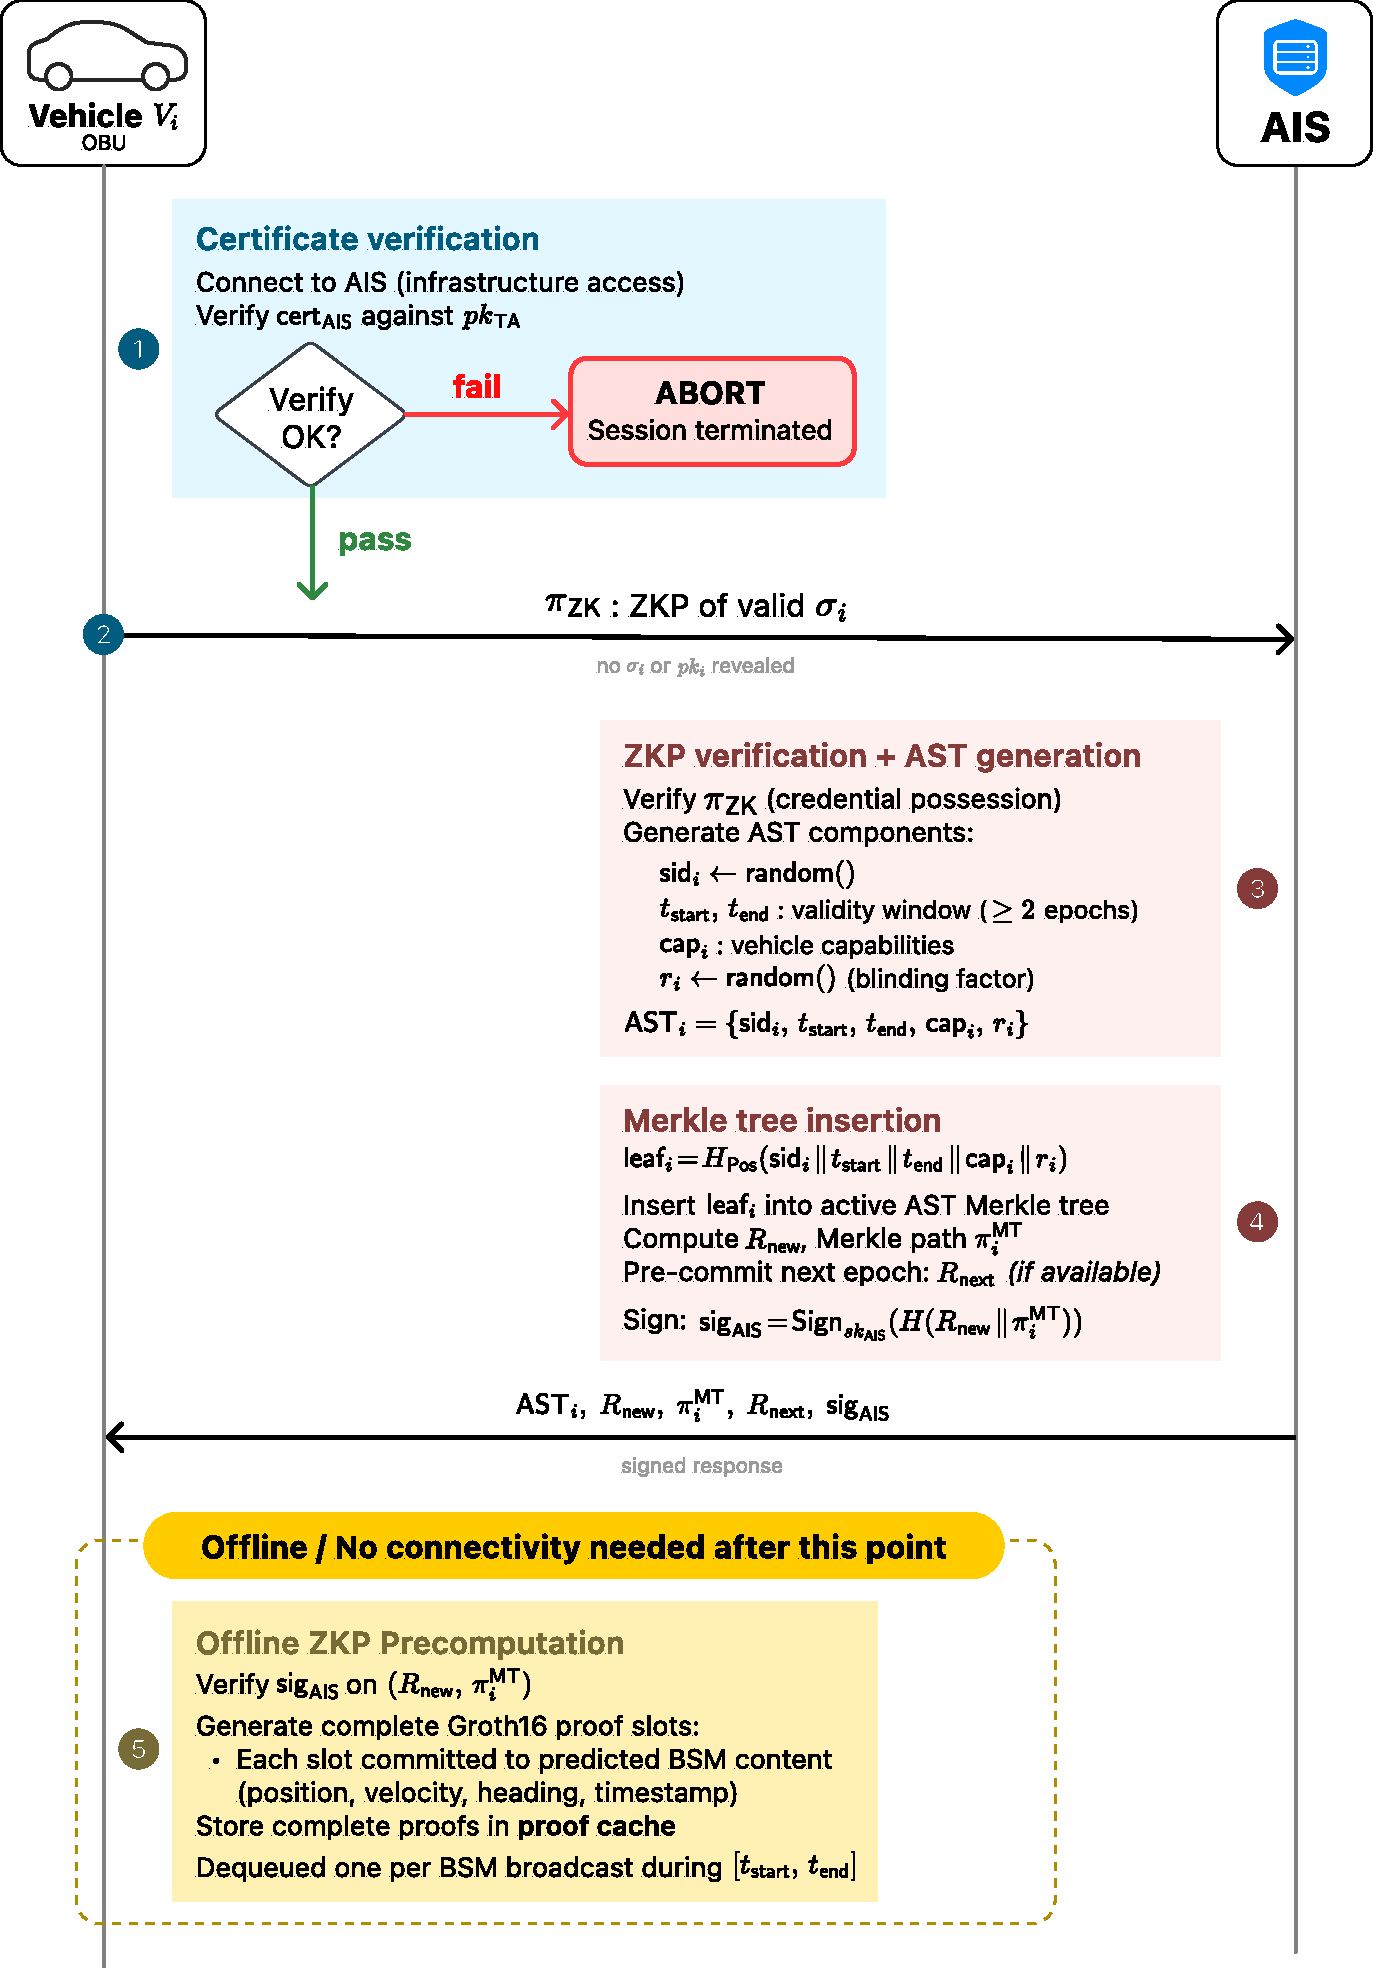
\includegraphics[width=\linewidth]{assets/phase2.pdf}
    \caption{Phase 2: AST acquisition. $V_i$ verifies the AIS certificate, presents
    a ZKP of credential possession, and receives an AST with Merkle path
    $\pi^{MT}_i$. Complete Groth16 proof slots are precomputed offline and stored
    in the proof-slot cache before the next driving segment.}
    \label{fig:phase2}
\end{figure}

\begin{algorithm}[t]
\caption{AST Acquisition and Offline Precomputation --- Phase 2 (Periodic)}
\label{alg:ast_acquisition}
\begin{algorithmic}[1]
\REQUIRE $(sk_i, \sigma_i, pk_{TA})$, proving key $\mathsf{pk}$, cache capacity $N_{\mathit{cache}}$
\ENSURE Proof cache $\mathcal{C}$ filled with $N_{\mathit{cache}}$ complete proof slots; current root $R$ stored
\STATE Connect to AIS via available infrastructure (RSU / cellular / Wi-Fi)
\STATE Retrieve $\mathsf{cert}_{AIS} = (pk_{AIS},\; \mathsf{validity},\; \mathsf{sig}_{TA})$ from AIS
\IF{$\mathsf{Verify}_{pk_{TA}}(\mathsf{cert}_{AIS}) = 0$}
    \STATE \textbf{abort} and report incident to TA
\ENDIF
\STATE $\pi_{\sigma} \leftarrow \mathsf{Prove}(\mathsf{pk},\; \emptyset,\; \sigma_i)$
    \hfill \COMMENT{ZKP of credential possession}
\STATE Send $\pi_{\sigma}$ to AIS; AIS verifies and issues $\mathsf{AST}_i$
\STATE \quad $\mathsf{leaf}_i \leftarrow H_{\mathit{Poseidon}}(sid_i \;\|\; t_{\mathit{start}} \;\|\; t_{\mathit{end}} \;\|\; \mathit{cap}_i \;\|\; r_i)$
\STATE Receive $(R_{\mathit{new}},\; \pi^{MT}_i,\; \mathsf{sig}_{AIS},\; R_{\mathit{next}})$ from AIS
\IF{$\mathsf{Verify}_{pk_{AIS}}\!\bigl(\mathsf{sig}_{AIS},\; H(R_{\mathit{new}} \;\|\; \pi^{MT}_i)\bigr) = 0$}
    \STATE \textbf{abort}
\ENDIF
\STATE Store $(\mathsf{AST}_i,\; \pi^{MT}_i,\; R_{\mathit{new}},\; R_{\mathit{next}})$ in OBU secure storage
\FOR{$s \leftarrow 1$ \TO $N_{\mathit{cache}}$}
    \STATE $(m^{(s)}_{\mathit{pred}},\; t^{(s)}_{\mathit{pred}}) \leftarrow \mathsf{PredictBSM}(s)$
        \hfill \COMMENT{GPS/IMU-based trajectory prediction}
    \STATE $h^{(s)}_m \leftarrow H_{\mathit{Poseidon}}(m^{(s)}_{\mathit{pred}} \| t^{(s)}_{\mathit{pred}})$
    \STATE $\pi^{(s)} \leftarrow \mathsf{Groth16.Prove}(\mathsf{pk},\; (R_{\mathit{new}},\; t^{(s)}_{\mathit{pred}},\; h^{(s)}_m),\; (\mathsf{AST}_i,\; \pi^{MT}_i,\; m^{(s)}_{\mathit{pred}}))$
    \STATE Append $(\pi^{(s)},\; h^{(s)}_m,\; t^{(s)}_{\mathit{pred}})$ to proof cache $\mathcal{C}$
\ENDFOR
\STATE Mark all slots in $\mathcal{C}$ as bound to root $R_{\mathit{new}}$
\end{algorithmic}
\end{algorithm}

\subsubsection{Phase 3: Online V2V Authentication (Per Message)}
When $V_i$ broadcasts safety message $m$ at time $t_{\mathit{cur}}$
(Fig.~\ref{fig:phase3}):
\begin{enumerate}
    \item $V_i$ dequeues the next proof slot $(\pi^{(s)}, h^{(s)}_m,
    t^{(s)}_{\mathit{pred}})$ from its cache. This operation is $< 0.01$\,ms.
    \item $V_i$ computes $h_m = H_{\mathit{Poseidon}}(m \| t_{\mathit{cur}})$ to
    verify prediction accuracy. If $h_m \neq h^{(s)}_m$ (i.e., the actual BSM
    content deviates beyond GPS tolerance from the pre-committed content), the slot
    is discarded and the next slot is tried; otherwise the slot is valid.
    \item The pre-generated proof $\pi^{(s)}$ already proves:
    \begin{equation}
    \begin{aligned}
        \text{``I know } & \mathsf{AST}_i \text{ and } \pi^{MT}_i \text{ such that:} \\
        & (1)\ \mathsf{Verify}_{MT}(\pi^{MT}_i, \mathsf{leaf}_i, R) = 1 \\
        & (2)\ t_{start} \leq t_{\mathit{pred}} \leq t_{end} \\
        & (3)\ h^{(s)}_m = H_{Poseidon}(m^{(s)}_{\mathit{pred}} \| t^{(s)}_{\mathit{pred}}) \text{''}
    \end{aligned}
    \end{equation}
    Public inputs: $(R,\; t^{(s)}_{\mathit{pred}},\; h^{(s)}_m)$. No proof
    computation occurs online.
    \item $V_i$ broadcasts $(m,\ t_{\mathit{cur}},\ \pi^{(s)},\ R)$. The verifier
    independently recomputes $H_{\mathit{Poseidon}}(m \| t_{\mathit{cur}})$ and
    checks it against $h^{(s)}_m$ in the proof's public inputs.
\end{enumerate}

The entire online phase is dominated by step~(2): one Poseidon-2 hash evaluation
(0.437\,ms, directly measured). No elliptic curve operations occur online---the
proof is already complete. Position prediction accuracy of $<3$\,m at highway
speeds (see Section~\ref{sec:bench_cache}) ensures slots are consumed without
discarding under normal driving.

\begin{figure}[t]
    \centering
    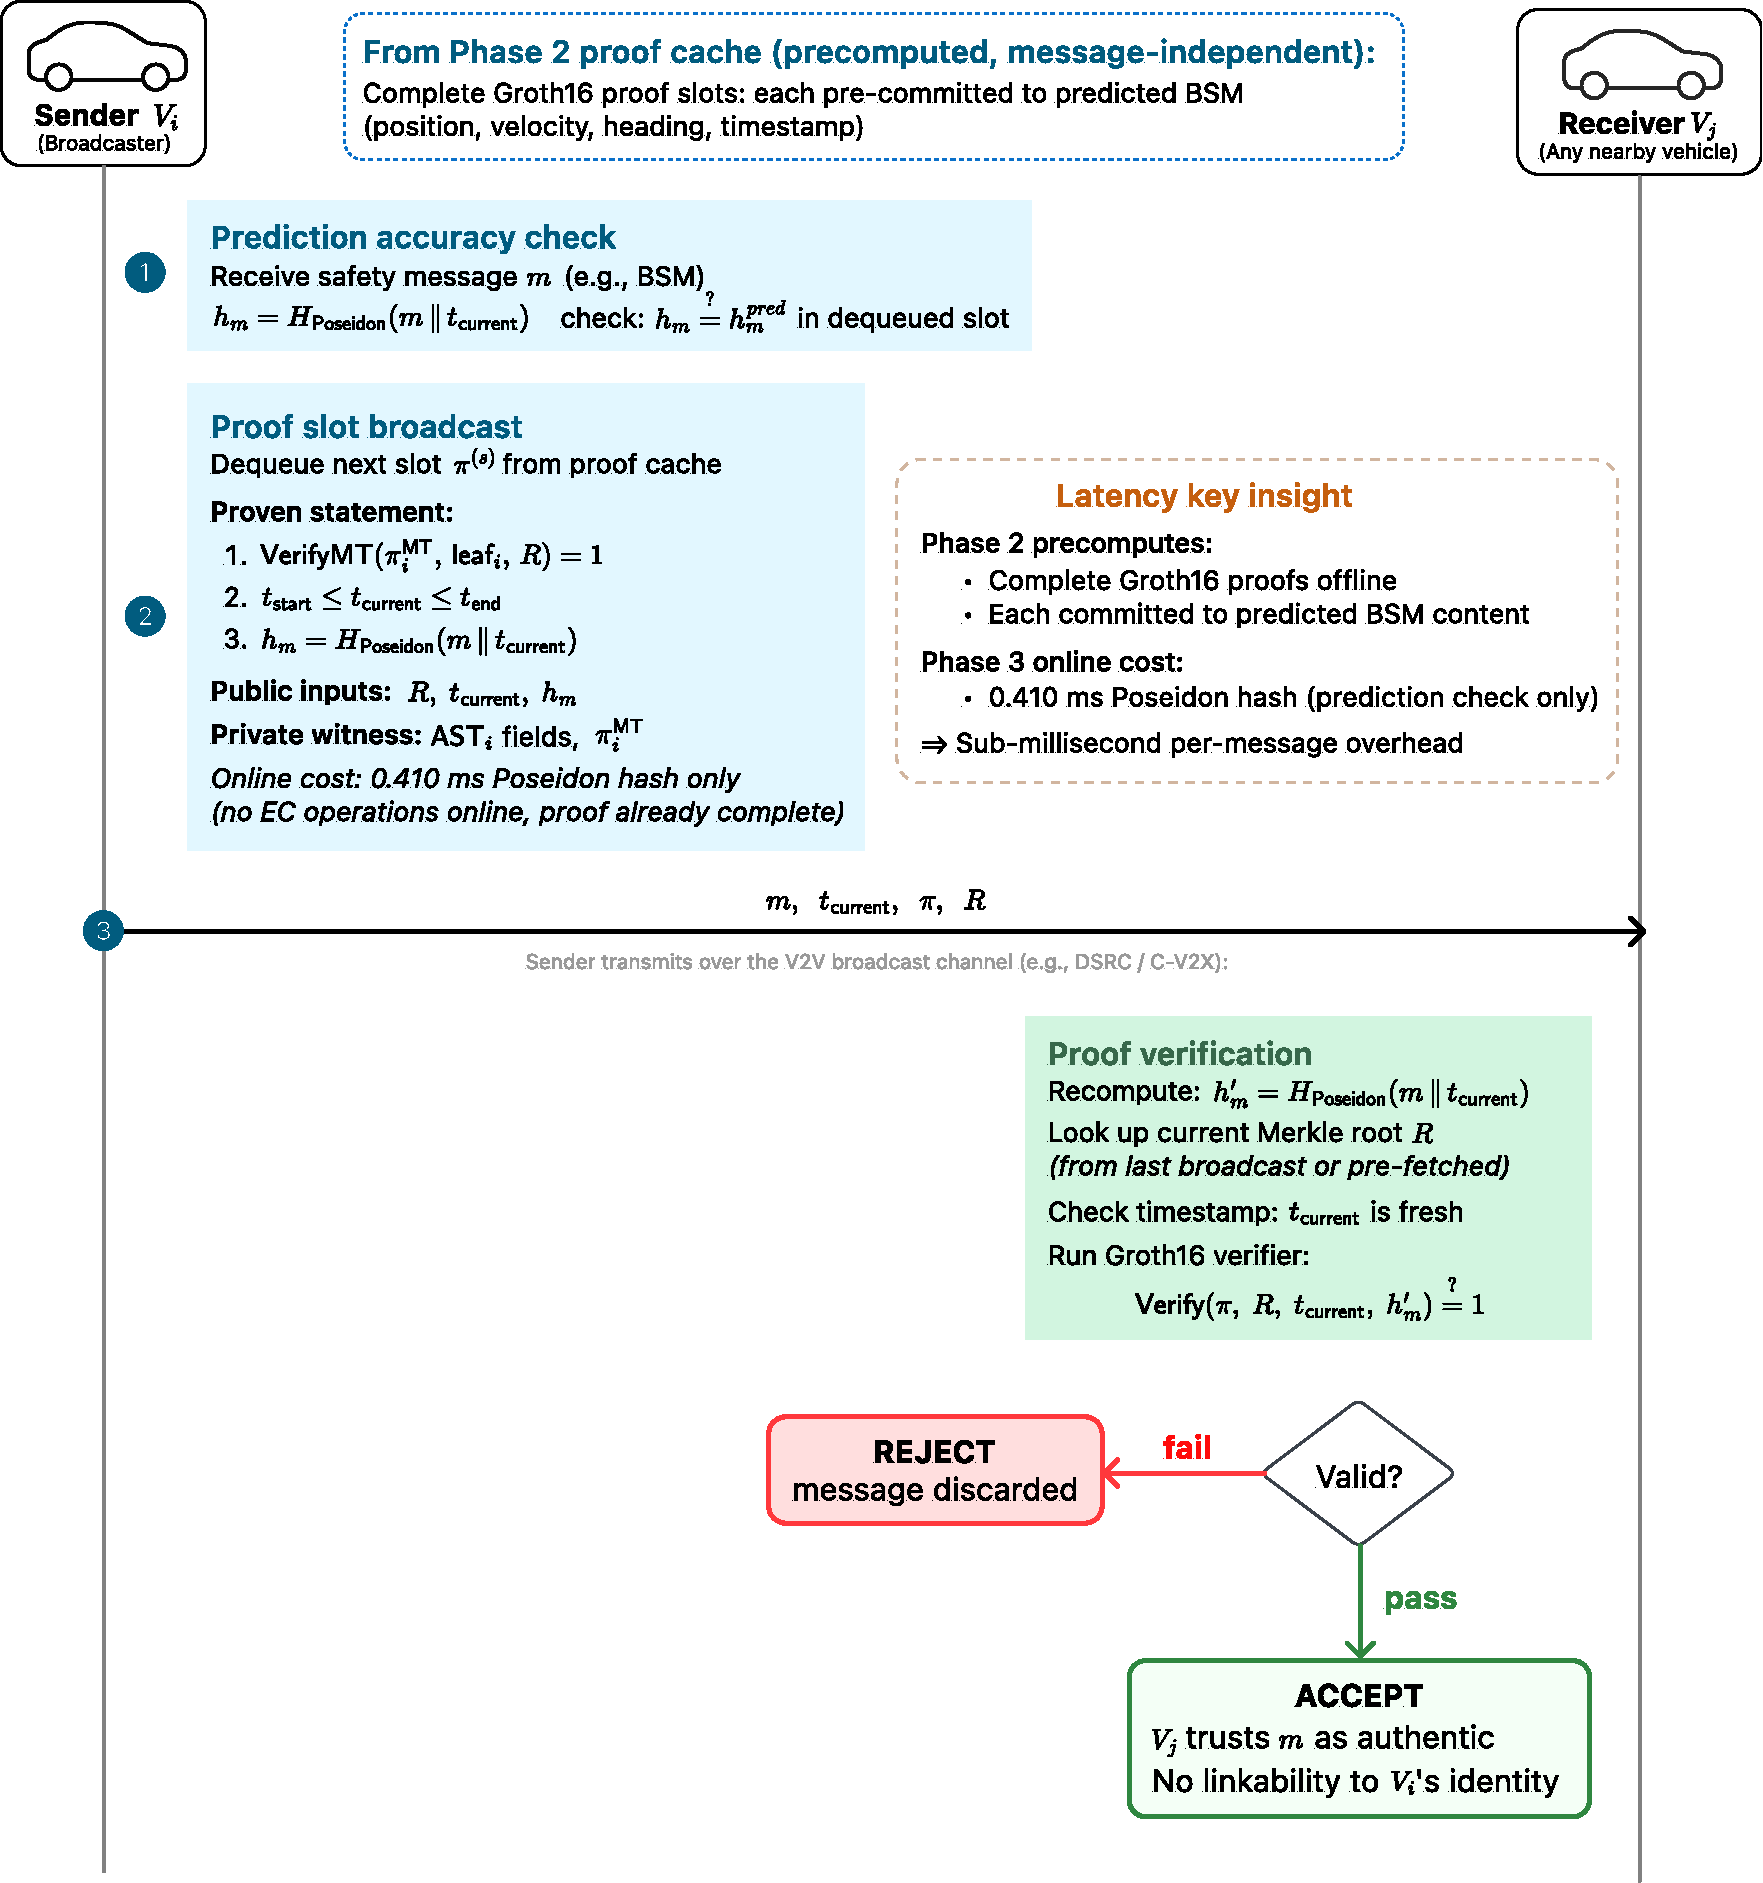
\includegraphics[width=\linewidth]{assets/phase3.pdf}
    \caption{Phase 3: Online V2V authentication. $V_P$ dequeues a pre-generated
    proof slot and computes $h_m = H_{\text{Poseidon}}(m \| t_{\text{current}})$
    to confirm prediction accuracy. No elliptic curve operations occur online. The
    tuple $(m, t_{\text{current}}, \pi, R)$ is broadcast over the V2V channel with
    total online cost 0.439\,ms.}
    \label{fig:phase3}
\end{figure}

\begin{algorithm}[t]
\caption{Online Proof Broadcast (Phase 3)}
\label{alg:online_proof}
\begin{algorithmic}[1]
\REQUIRE Proof cache $\mathcal{C} = \{(\pi^{(s)}, h^{(s)}_m, t^{(s)}_{\mathit{pred}})\}$, message $m$, timestamp $t_{\mathit{cur}}$
\ENSURE Broadcast authenticated BSM or discard slot
\STATE Dequeue next slot $(\pi^{(s)}, h^{(s)}_m, t^{(s)}_{\mathit{pred}})$ from $\mathcal{C}$
    \hfill \COMMENT{$< 0.01$\,ms}
\STATE $h_m \leftarrow H_{\mathrm{Poseidon}}(m \| t_{\mathit{cur}})$
    \hfill \COMMENT{$0.437$\,ms, irreducible online cost}
\IF{$h_m \neq h^{(s)}_m$}
    \STATE Discard slot; try next slot \hfill \COMMENT{prediction miss; rare at highway speeds}
\ENDIF
\STATE Broadcast $(m,\; t_{\mathit{cur}},\; \pi^{(s)},\; R)$
    \hfill \COMMENT{proof already complete; no EC ops online}
\end{algorithmic}
\end{algorithm}

\subsubsection{Phase 4: Batch Verification (Receiver Side)}
Verifier vehicle $V_V$ receiving multiple authenticated messages (Fig.~\ref{fig:phase4}):
\begin{enumerate}
    \item $V_V$ checks that the Merkle root $R$ in each message matches
    $R_{current}$ (or $R_{prev}$ during $T_{grace}$). Messages with unrecognised
    roots are immediately discarded.
    \item $V_V$ applies priority filtering: emergency-class messages are
    individually verified immediately; standard BSMs are buffered for batch
    verification.
    \item $V_V$ collects $k$ standard proofs within window $T_{window}$
    (50--100\,ms).
    \item $V_V$ performs batched Groth16 verification. For individual verification:
    \begin{equation}
        e(A_j, B_j) = e(\alpha, \beta) \cdot e(L_j, \gamma) \cdot e(C_j, \delta)
    \end{equation}
    For batch verification of $k$ proofs, the verifier samples random scalars
    $\rho_1, \ldots, \rho_k$ and checks:
    \begin{equation}
        \prod_{j=1}^{k} e(A_j, B_j)^{\rho_j} = e(\alpha, \beta)^{\sum \rho_j}
        \cdot \prod_{j=1}^{k} e(L_j, \gamma)^{\rho_j}
        \cdot \prod_{j=1}^{k} e(C_j, \delta)^{\rho_j}
    \end{equation}
    Using multi-scalar multiplication, this reduces pairings from $3k$
    (individual) to $k+3$ (batched).
    \item If batch verification fails, $V_V$ applies the Divide-and-Conquer
    Verifier (DCV, Algorithm~\ref{alg:dcv_fallback}) to identify invalid
    proof(s) in $O(w \log k)$ sub-batch operations rather than $O(k)$ individual
    verifications, where $w$ is the number of invalid proofs.
\end{enumerate}

\begin{figure}[t]
    \centering
    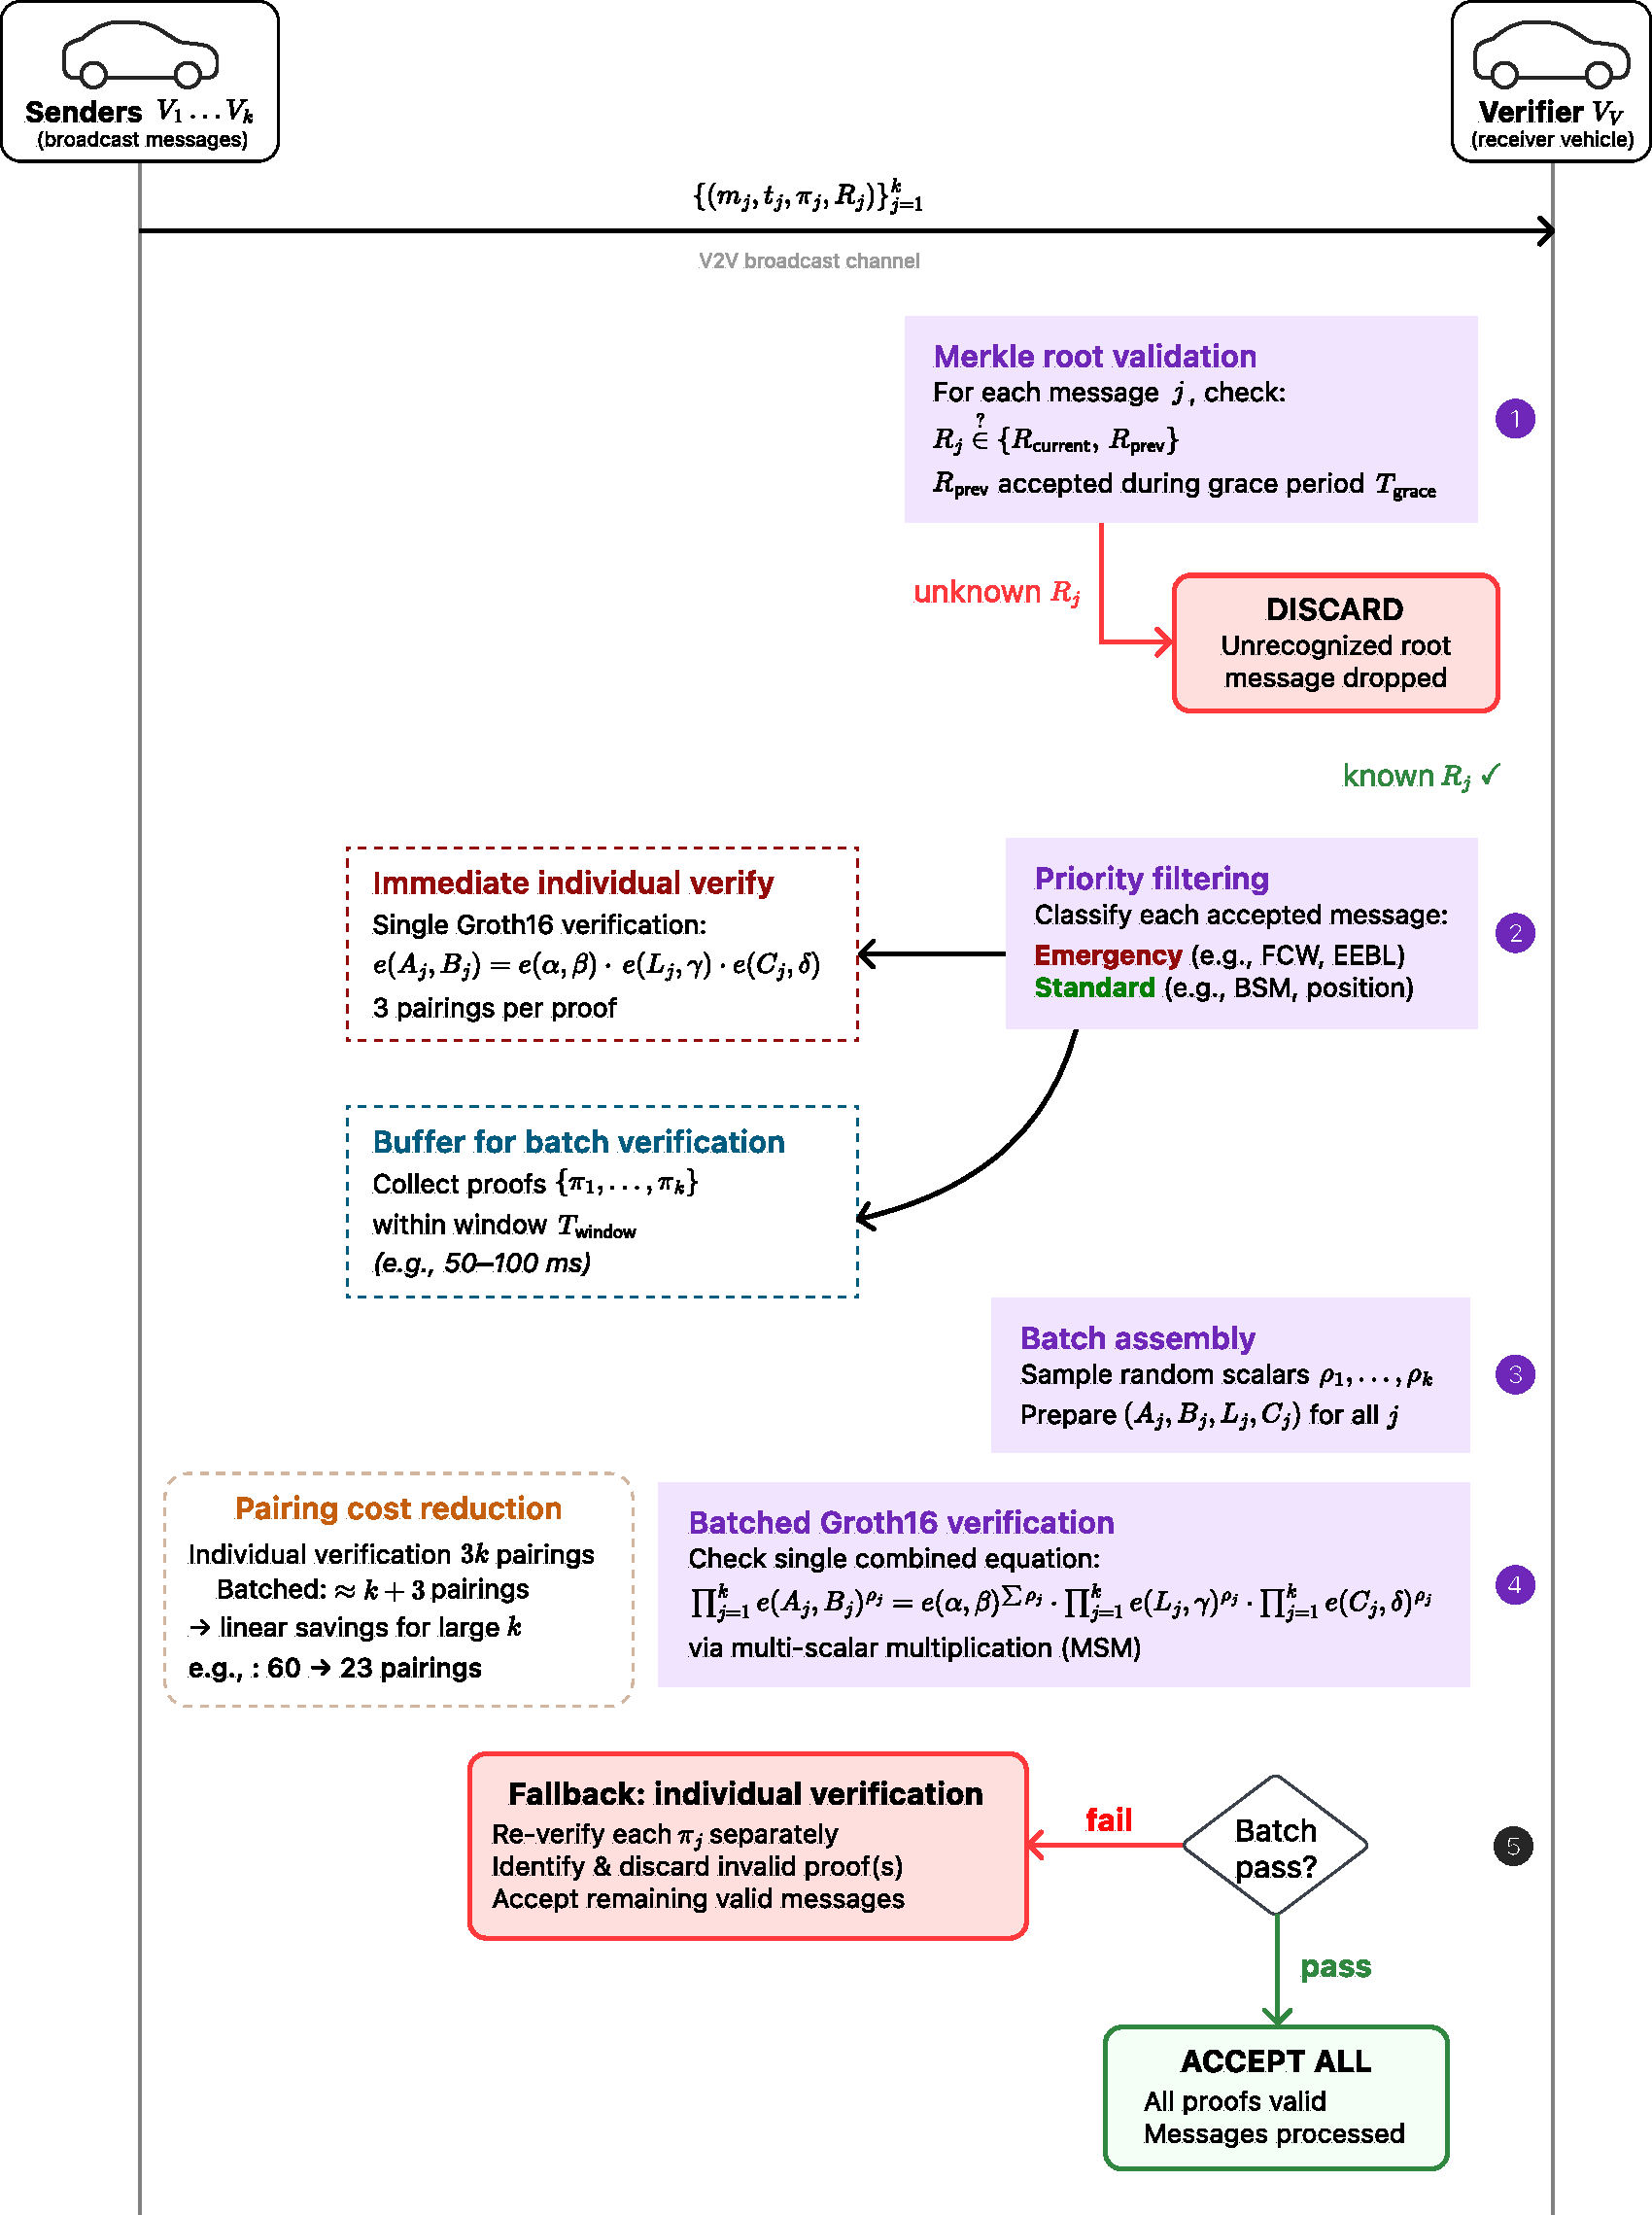
\includegraphics[width=\linewidth]{assets/phase4.pdf}
    \caption{Phase 4: Batch verification. $V_V$ filters incoming proofs by Merkle
    root validity, immediately verifies high-priority messages individually, and
    aggregates standard BSMs for a single batched Groth16 pairing check, reducing
    verification cost from $3k$ to $\approx k+3$ pairings for a batch of $k$ proofs.}
    \label{fig:phase4}
\end{figure}

\begin{algorithm}[t]
\caption{True Batch Groth16 Verification (Phase 4 / Bellare--Garay--Rabin~\cite{bellare1998})}
\label{alg:batch_verify}
\begin{algorithmic}[1]
\REQUIRE Proofs $\{(A_j,B_j,C_j)\}_{j=1}^{k}$, public signals $\{\mathbf{pub}_j\}$, $\mathsf{vk}=(\alpha,\beta,\gamma,\delta,\mathit{IC})$
\ENSURE \textbf{accept} or \textbf{reject}
\FOR{each $j = 1$ to $k$}
  \IF{$R_j \neq R_{\mathit{current}}$}  \RETURN \textbf{reject}  \ENDIF
\ENDFOR
\FOR{each $j = 1$ to $k$}
  \STATE Sample $\rho_j \xleftarrow{\$} \mathbb{Z}_p^*$
\ENDFOR
\STATE $\mathit{aggAlpha} \leftarrow \bigl(\textstyle\sum_j \rho_j\bigr)\cdot\alpha$
\FOR{each $j = 1$ to $k$}
  \STATE $L_j \leftarrow \mathit{IC}[0] + \sum_{i} \mathbf{pub}_j[i]\cdot\mathit{IC}[i+1]$
\ENDFOR
\STATE $\mathit{aggL} \leftarrow \sum_j \rho_j \cdot L_j$;\quad
       $\mathit{aggC} \leftarrow \sum_j \rho_j \cdot C_j$
\STATE Check: $\prod_j e(\rho_j A_j, B_j)\cdot e(-\mathit{aggAlpha},\beta)\cdot e(-\mathit{aggL},\gamma)\cdot e(-\mathit{aggC},\delta) \stackrel{?}{=} 1_{\mathbb{G}_T}$
\IF{check passes}  \RETURN \textbf{accept}
\ELSE  \STATE \CALL{DCVFallback}{$\{(A_j,B_j,C_j,\mathbf{pub}_j)\}_{j=1}^k$, $\mathsf{vk}$}
    \hfill \COMMENT{Algorithm~\ref{alg:dcv_fallback}}
\ENDIF
\end{algorithmic}
\end{algorithm}

\begin{algorithm}[t]
\caption{DCV Fallback: Divide-and-Conquer Invalid Proof Isolation~\cite{ferrara2008finding}}
\label{alg:dcv_fallback}
\begin{algorithmic}[1]
\REQUIRE Proof set $\mathcal{P} = \{(A_j,B_j,C_j,\mathbf{pub}_j)\}_{j=1}^{k}$, $\mathsf{vk}$
\ENSURE Set $\mathcal{B} \subseteq \mathcal{P}$ of all invalid proofs
\IF{$|\mathcal{P}| = 1$}
    \IF{\CALL{IndividualVerify}{$\mathcal{P}[1]$, $\mathsf{vk}$} $= 0$}
        \RETURN $\mathcal{P}$ \hfill \COMMENT{base case: singleton invalid}
    \ELSE\ \RETURN $\emptyset$
    \ENDIF
\ENDIF
\STATE $\mathcal{P}_L \leftarrow \mathcal{P}[1 \mathinner{..} \lfloor k/2 \rfloor]$;\quad
       $\mathcal{P}_R \leftarrow \mathcal{P}[\lfloor k/2 \rfloor + 1 \mathinner{..} k]$
\STATE $\mathcal{B} \leftarrow \emptyset$
\IF{\CALL{BatchVerify}{$\mathcal{P}_L$, $\mathsf{vk}$} $= 0$}
    \STATE $\mathcal{B} \leftarrow \mathcal{B} \cup$ \CALL{DCVFallback}{$\mathcal{P}_L$, $\mathsf{vk}$}
\ENDIF
\IF{\CALL{BatchVerify}{$\mathcal{P}_R$, $\mathsf{vk}$} $= 0$}
    \STATE $\mathcal{B} \leftarrow \mathcal{B} \cup$ \CALL{DCVFallback}{$\mathcal{P}_R$, $\mathsf{vk}$}
\ENDIF
\RETURN $\mathcal{B}$
\end{algorithmic}
\end{algorithm}

\noindent\textbf{DCV complexity in the Groth16 setting.}
For $k$ proofs and $w$ invalid proofs, DCV performs at most $2w\lceil\log_2(k/w)\rceil$
sub-batch verifications~\cite{ferrara2008finding}. Each sub-batch of size $k'$ costs
$(k'+3)$ pairings, so total pairing count is
$O(w \log(k/w) \cdot (k/w + 3)) = O(k + w \log k)$.
At $k=30$, $w=1$ (single adversarial injection): DCV costs $\approx 5$ sub-batch
operations ($\approx 500$\,ms on RPi~4) versus $30$ individual verifications
($2{,}100$\,ms) under naive fallback---a \textbf{4.2$\times$ improvement} in
worst-case fallback cost. We additionally pre-screen each incoming proof for valid
$\mathbb{G}_1$/$\mathbb{G}_2$ curve membership and timestamp freshness before
batching ($< 0.1$\,ms per proof), eliminating malformed injections before they enter
Algorithm~\ref{alg:batch_verify}.

\subsection{Revocation Mechanism}

When the TA determines that a vehicle should be revoked:
\begin{enumerate}
    \item The TA instructs the AIS to remove $\mathsf{leaf}_i$ from the active
    Merkle tree.
    \item The AIS recomputes the Merkle tree and publishes the updated root
    $R_{new}$.
    \item Vehicles periodically download the updated root during infrastructure
    contact.
    \item Any proof generated with a revoked AST will fail verification because
    the leaf is no longer in the tree.
\end{enumerate}

The revocation overhead is $O(\log n)$ per vehicle versus $O(n)$ for a full CRL.
Fig.~\ref{fig:merkle_revoc} illustrates this for a depth-3 tree ($n=8$): revoking
$\mathtt{AST_3}$ recomputes exactly $\lceil\log_2 8\rceil = 3$ nodes along the path
to the root, broadcasting only a 32-byte new root $R_{\text{new}}$.

\begin{figure}[t]
    \centering
    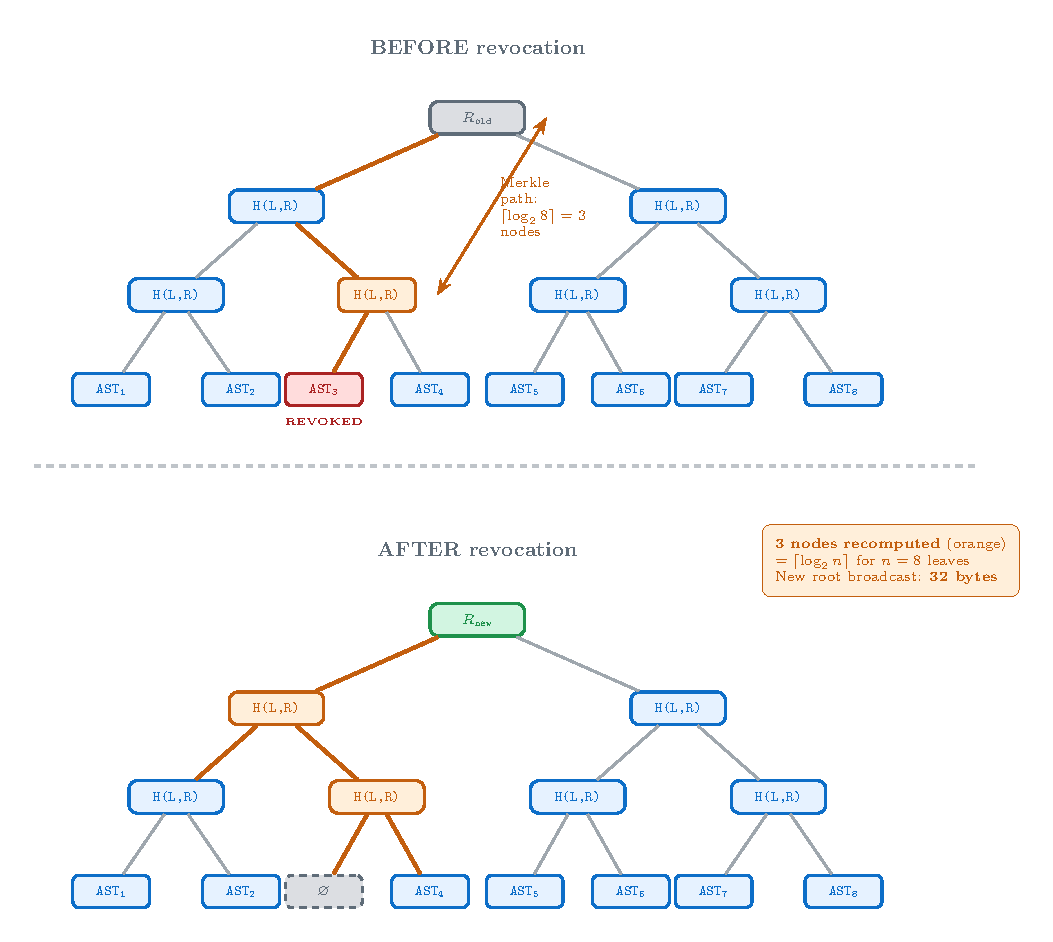
\includegraphics[width=\linewidth]{assets/merkle_tree_revoc.pdf}
    \caption{Merkle tree revocation: before (above) and after (below) revoking
    $\mathtt{AST_3}$ from an $n=8$ leaf tree. Only the $\lceil\log_2 n\rceil = 3$
    nodes along the path to the root (orange) are recomputed; all other subtrees
    remain unchanged (blue). The new 32-byte root $R_{\text{new}}$ (green) is
    broadcast to all verifiers.}
    \label{fig:merkle_revoc}
\end{figure}

\subsection{Resilience Under Real-World Channel Conditions}
\label{sec:noise}

Highway V2V channels exhibit three significant impairments not addressed by most
ZKP authentication proposals.

\subsubsection{Packet Loss and Authentication Success Rate}

IEEE 802.11p DSRC field measurements show PLR of 10--40\% at 150--300\,m range
under NLoS conditions~\cite{ramadan2025}. For a verifier $V_V$ receiving from
prover $V_P$ at PLR $\rho$, the expected batch size is
$k_{recv} = k_{sent} \cdot (1 - \rho)$.
Since proofs are independently transmitted, packet loss reduces batch size but does
not corrupt the batch check for received proofs. The authentication success rate is:
\begin{equation}
    \mathsf{ASR} = (1 - \rho) \cdot \Pr[\text{ZKP valid}]
\end{equation}
For honest provers, $\Pr[\text{ZKP valid}]=1$, so ASR is bounded by the channel
PLR---the cryptographic overhead introduces \emph{no additional failure modes}.

\subsubsection{Channel Congestion Under Dense Traffic}

At $>$100 vehicles/km, the 802.11p EDCA mechanism becomes saturated under 10\,Hz
BSM broadcasting. ULP-V2V-Auth's per-message overhead of $\approx$224\,bytes
(128\,B proof $+$ 96\,B public inputs $+$ message hash) is approximately $2\times$
smaller than SCMS's 400--600\,bytes (signature $+$ pseudonym certificate), directly
reducing channel load and collision probability. The Receiver Module's priority
filtering (Section~\ref{sec:concurrent}) ensures emergency BSMs receive deterministic
authentication latency independent of batch backpressure, consistent with EDCA
priority at the MAC layer.

\subsubsection{Infrastructure Connectivity for AST Acquisition}

With a proof cache sized for $N_{cache}=6000$ slots (10 minutes at 10\,Hz) and RSU
contacts every 30--100\,s on typical highway deployments, the expected time until
cache exhaustion far exceeds typical infrastructure gap durations. In the rare case
of cache exhaustion, the vehicle enters degraded mode (Section~\ref{sec:epoch}),
continuing to verify and react to authenticated messages from others while ceasing
transmission, preserving cooperative awareness.
